% Figure: overconfidence factor of a record rebuilt each round from its readers' posteriors (prop:hie-literal-records,
% tab:hie-records) under the four aggregation rules (E), (U), (A), (P), rounds t = 1, ..., 8. Static scalar latent
% with prior precision Lambda_o = 1, n = 3 members of unit information (Lambda^o = 3). oc(t) = MSE(t) Lambda_z(t)
% from the closed forms of tab:hie-records:
%   (E) oc = 1;
%   (U) oc = (Lambda_o + t^2 Lambda^o)/(Lambda_o + t Lambda^o);
%   (A) oc = (Lambda_o + t^2 Lambda^o/n^2)/(Lambda_o + t Lambda^o/n);
%   (P) oc = [Lambda_o n^(2t) (n-1)^2 + Lambda^o (n^t-1)^2]/[Lambda_o n^t (n-1) + Lambda^o (n^t-1)]^2
%            times Lambda_z = n^t Lambda_o + Lambda^o (n^t-1)/(n-1).
% Double precision. Iterating the four rules on explicit coefficient vectors over (Lambda_o m_o, h_1, h_2, h_3)
% reproduces every precision, mean-square error and oc of the closed forms to 4.3e-16. At t = 8: Lambda_z = 4, 25,
% 9, 16401; mean-square errors 0.2500, 0.3088, 0.2757, 0.2800; oc = 1, 7.72, 2.48, 4.59e3, the values of
% chk:hie-literal. (U) has oc = 1 at t = 1 (exact after one round); (A) has oc = 1 exactly at t = n = 3, below one
% before (0.667 and 0.778) and above one after; (P) grows like n^t. Over t = 1, ..., 8 every rule keeps the
% mean-square error between 1/4 and 1/3, so the growth of oc is the growth of the claimed precision. Shaded band:
% oc < 1. Data are embedded as computed.
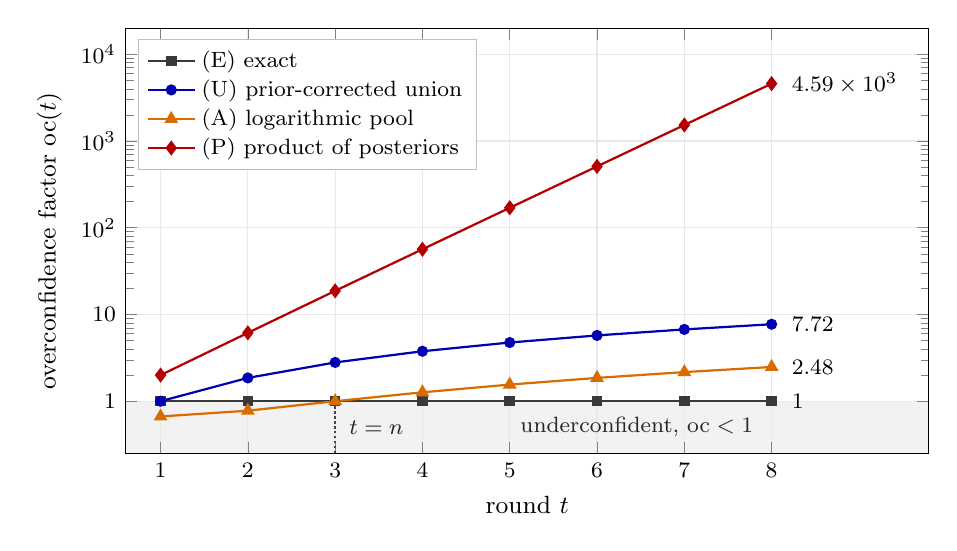
\begin{tikzpicture}
  \begin{semilogyaxis}[name=oc, scale only axis, width=10.2cm, height=5.4cm, set layers,
      xmin=0.6, xmax=9.8, ymin=0.25, ymax=2e4,
      xtick={1,...,8}, ytick={1,10,100,1000,10000}, yticklabels={$1$,$10$,$10^2$,$10^3$,$10^4$},
      xlabel={round $t$}, ylabel={overconfidence factor $\mathrm{oc}(t)$},
      grid=major, grid style={gray!18},
      legend style={font=\footnotesize, at={(0.015,0.975)}, anchor=north west, draw=gray!50, fill=white,
        cells={anchor=west}, row sep=-1pt},
      every axis label/.style={font=\small}, tick label style={font=\footnotesize}]
    \begin{pgfonlayer}{axis background}
      \fill[gray!10] (axis cs:0.6,0.25) rectangle (axis cs:9.8,1);
    \end{pgfonlayer}
    \addplot[gray!45!black, thick, mark=square*, mark size=1.5pt] coordinates {(1,1) (2,1) (3,1) (4,1) (5,1) (6,1) (7,1) (8,1)};
    \addlegendentry{(E) exact}
    \addplot[blue!70!black, thick, mark=*, mark size=1.6pt] coordinates {(1,1) (2,1.8571) (3,2.8) (4,3.7692) (5,4.75) (6,5.7368) (7,6.7273) (8,7.72)};
    \addlegendentry{(U) prior-corrected union}
    \addplot[orange!85!black, thick, mark=triangle*, mark size=2.1pt] coordinates {(1,0.66667) (2,0.77778) (3,1) (4,1.2667) (5,1.5556) (6,1.8571) (7,2.1667) (8,2.4815)};
    \addlegendentry{(A) logarithmic pool}
    \addplot[red!70!black, thick, mark=diamond*, mark size=2.1pt] coordinates {(1,2) (2,6.1429) (3,18.727) (4,56.522) (5,169.92) (6,510.12) (7,1530.7) (8,4592.5)};
    \addlegendentry{(P) product of posteriors}
    % values at t = 8
    \node[font=\footnotesize, anchor=west] at (axis cs:8.12,4592.5) {$4.59\times10^3$};
    \node[font=\footnotesize, anchor=west] at (axis cs:8.12,7.72) {$7.72$};
    \node[font=\footnotesize, anchor=west] at (axis cs:8.12,2.4815) {$2.48$};
    \node[font=\footnotesize, anchor=west] at (axis cs:8.12,1) {$1$};
    % (A) is calibrated at t = n = 3
    \draw[gray!55!black, densely dotted, thick] (axis cs:3,0.25) -- (axis cs:3,1);
    \node[font=\footnotesize, gray!30!black, anchor=west] at (axis cs:3.05,0.5) {$t=n$};
    \node[font=\footnotesize, gray!30!black, anchor=east] at (axis cs:7.9,0.5) {underconfident, $\mathrm{oc}<1$};
  \end{semilogyaxis}
\end{tikzpicture}
